\chapter{Conclusioni} % (fold)

Il modello è stato progettato e realizzato per svolgere la segmentazione d'immagini di femori fetali \cite{abstract1} \cite{abstract2}.
L'utilizzo del modello permette l'automatizzazione di un compito che altrimenti richiederebbe lo sforzo e il tempo di un 
professionista che così può svolgere altre attività meno monotone.
Nello specifico il modello è stato utilizzato per automatizzare l'estrazione dei pixel relativi al femore di un feto 
nelle settimane 35-37 di gestazione. 
I pixel estratti venivano processati per estrarne la luminosità che nelle analisi ecografiche corrisponde 
alla \textbf{densità minerale ossea} o \textbf{bone mineral density}(BMD) del femore fetale
per correlarlo ai dati relativi al peso di nascita.

È stato rilevato un tendenza di correlazione debole tra luminosit\`a e peso alla nascita. (\autoref{fig:correlazione tra luminosità e peso alla nascita})

\begin{figure}[H]
    \centering
    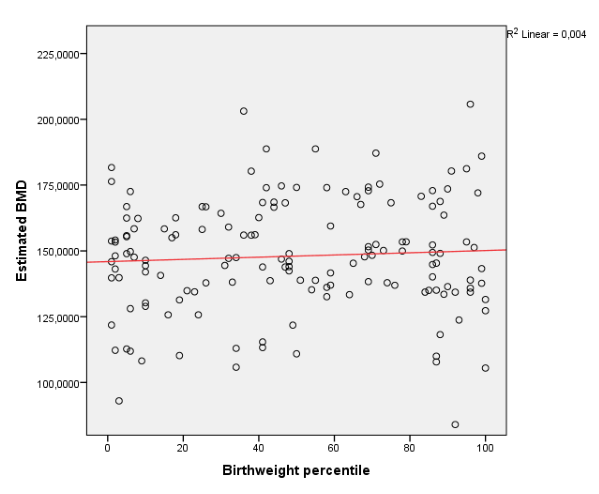
\includegraphics[width=0.6\columnwidth]{Immagini/correlation_weight_abstract.png}
    \caption{Correlazione tra luminosità e peso alla nascita}
    \label{fig:correlazione tra luminosità e peso alla nascita}
\end{figure}


La rete neurale si è dimostrata capace di riconoscere i pixel contenenti dati relativi all'area del femore, inoltre i dati prodotti dalla rete hanno portato a tenere in considerazione 
l'utilizzo della rete per analisi successive.